% \todo{Erstellen = erstellen, aktualisieren, löschen}
\begin{description}[leftmargin=0.5cm,style=nextline]
% client push
\item[Szenario C0 -- Client push:]
Der Client erstellt einen Adressbucheintrag, hat den Status \sc{online} und der Server ist erreichbar. Sowohl Anfrage als auch Antwort sind erfolgreich. Der Kontakt wird erfolgreich erstellt.\\
\item[Szenario C1 -- Client push:]
Der Client erstellt einen Adressbucheintrag, hat den Status \sc{offline} und der Server ist nicht erreichbar. Die Anfrage schlägt fehl.\\
\item[Szenario C2 -- Client push:]
Der Client erstellt einen Adressbucheintrag und hat den Status \sc{online}. Die Anfrage wird gestartet und währenddessen bricht die Internetverbindung ab. Die Anfrage `wartet` bis ein Timeout getriggert wird und schlägt dann fehl. Wärend des Wartens ist der Client blockiert.\\
% \item[Szenario C3 -- Client push:]
% Der Client erstellt einen Adressbucheintrag und hat den Status \sc{online}. Die Anfrage wird gestartet und währenddessen bricht die Internetverbindung ab. Die Anfrage ist teilweise erfolgreich. Nur ein Teil der Telefonnummer kommen beim Server an.\\
% client pull / server push
\item[Szenario S0 -- Server push/Client pull:]
Der Client fordert eine Liste aller gespeicherten Kontakte vom Server an, hat den Status \sc{online} und der Server ist erreichbar. Sowohl Anfrage als auch Antwort sind erfolgreich. Die Liste wird komplett ausgeliefert.\\
\item[Szenario S1 -- Server push/Client pull:]
Der Client fordert eine Liste aller gespeicherten Kontakte vom Server an. Dieser hat den Status \sc{offline} und ist nicht erreichbar. Die Antwort schlägt fehl.\\
\item[Szenario S2 -- Server push/Client pull:]
Der Client fordert eine Liste aller gespeicherten Kontakte vom Server an und hat den Status \sc{online}.
Während der Server antwortet, bricht die Internetverbindung ab. Die Antwort `wartet` bis ein Timeout getriggert wird und schlägt dann fehl.
Wärend des Wartens ist der Client blockiert.\\
\item[Szenario S3 -- Server push/Client pull:]
Der Client fordert eine Liste aller gespeicherten Kontakte vom Server an und hat den Status \sc{online}.
Während der Server antwortet, bricht die Internetverbindung ab. Die Antwort ist teilweise erfolgreich.
Nur ein Teil der angefragten Daten kommt beim Client an.
\end{description}
%
%
In den obigen Szenarien wird nicht beschrieben warum die Verbindung zwischen den beiden Parteien abbricht. Dies kann verschiedene Gründe haben.
Um nur einige Beispiele zu nennen: Eine langsame Internetverbindung, oder eine Fahrt durch einen Tunnel kann ein Timeout während einer Aktion hervorrufen.
Ein auf einer Baustelle gekapptes Kabel oder ein Stromausfall kann zu zeitweise vollständigem Internetverlust führen.
Genausogut kann es jedoch sein, dass der Server kaputt oder nicht erreichbar ist. Es gibt meherere Gründe dafür, dass die beiden Parteien nicht mehr miteinander kommunizieren können.

Die Abbildung \ref{fig:szenarien} veranschaulicht die beschriebenen Situationen, die bei der Übertragung von Daten über das Netzwerk eintreten können.
Die Felder in lila beschreiben die Szenarien bei denen der Client etwas an den Server schickt.
Die blauen Felder auf der rechten Seite zeigen solche Szenarien, die eintreten können wenn der Server etwas an den Client sendet.
Die Sechsecke stehen für die Ausgangssituationen, die Kreise repräsentieren die Szenarien und die Rechtecke die daraus resultierenden Fälle.
\begin{figure}[H]
  \centering
  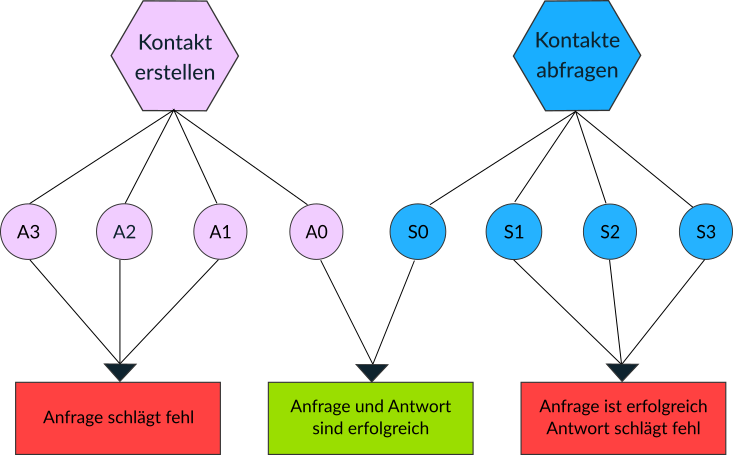
\includegraphics[width=0.8\textwidth]{Szenarien}
  \grayRule
  \caption{Szenarien bei der Datenübertragung über das Netzwerk}
  \label{fig:szenarien}
\end{figure}

%
% ERGEBNIS
%
\subsubsection*{Ergebnis}
Da die Szenarien \it{C0} und \it{S0}, die Szenarien \it{C1} und \it{C2} sowie die Szenazien \it{S1}, \it{S2} und \it{S3} zusammengefasst werden können, ergeben sich aus den sieben Szenarien die drei nun aufgezählten Fälle.
\begin{itemize}
  \item Fall a: Anfrage und Antwort sind erfolgreich.
  \item Fall b: Anfrage ist nicht erfolgreich
  \item Fall c: Anfrage ist erfolgreich, Antwort schlägt fehl
\end{itemize}